\section{Introduction}

In the realm of software engineering, meeting requirements encompasses both functional and non-functional aspects:
\begin{itemize}
    \item \textit{Functional requirements}: the software must effectively execute its intended purpose.
    \item \textit{Non-functional requirements}: 
        \begin{itemize}
            \item \textit{Usability}: the software should be user-friendly and intuitive.
            \item \textit{Safety}: it should maintain a secure environment for users and data.
            \item \textit{Security}: robust measures should be in place to protect against breaches and unauthorized access.
        \end{itemize}
\end{itemize}
Recognizing the significance of crafting inherently secure applications is pivotal for any proficient developer or software engineer. 
However, it's worth acknowledging that developing secure software presents formidable challenges.

Software must conform to the specified requirements. 
Not meeting a requirement results in a software bug. 
Failure to meet a security requirement creates a vulnerability. 
Exploiting a vulnerability to compromise the confidentiality, integrity, or availability (CIA) of a system is termed an exploit.

\begin{figure}[H]
    \centering
    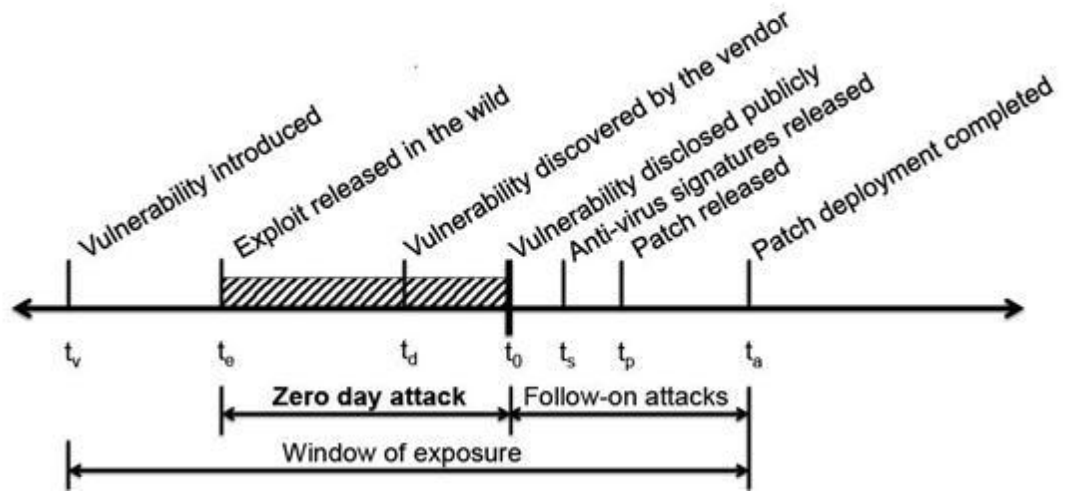
\includegraphics[width=1.0\linewidth]{images/vulnerability.png}
    \caption{Vulnerability lifecycle}
\end{figure}

\subsection{Principles of secure design}
\begin{enumerate}
    \item \textit{Minimize privileged access}: limit privileged access to the essential components.
    \item \textit{Keep it simple, stupid (KISS)}: embrace simplicity in design to reduce potential vulnerabilities.
    \item \textit{Immediate privilege discard}: promptly discard privileges, like transitioning from SUID to RUID, to mitigate potential security risks.
    \item \textit{Open design}: rely on openness rather than obscurity for security, aligning with Kerckhoffs' principle.
    \item \textit{Address concurrency and race conditions}: be vigilant about handling concurrency and race conditions, as they pose intricate security challenges.
    \item \textit{Fail-safe and default deny}: implement fail-safe mechanisms and default deny policies to enhance security posture.
    \item \textit{Avoid shared resources and untrusted libraries}: refrain from using shared resources like \texttt{mktemp} and \texttt{opt} against incorporating unknown or untrusted libraries into the system.
    \item \textit{Input and output filtering}: implement robust input and output filtering mechanisms to mitigate potential attack vectors.
    \item \textit{Use established cryptographic primitives}: avoid developing custom cryptographic primitives, password, or secret management code; instead, rely on audited and trusted cryptographic libraries.
    \item \textit{Trustworthy random number generation}: utilize reliable random number generators such as \texttt{/dev/[u]random} to ensure the integrity of cryptographic operations and secure communications.
\end{enumerate}

\paragraph*{Summary}
Bug-free software is an ideal that's practically unattainable. 
While not all bugs lead to vulnerabilities, achieving software devoid of vulnerabilities is a challenging task.
It's important to remember that vulnerabilities can exist without any working exploits targeting them.
Additionally, exercising caution with the SUID permission bit is crucial due to its potential security implications.